\documentclass[../../main.tex]{subfiles}
\begin{document}
\section{Successioni e Limiti}
Una \textbf{successione} è una legge che ad ogni numero naturale $n$ fa
corrispondere uno ed un solo numero reale $a_n$. Una successione è una funzione
di $\mathbb{N} in \R$.
\begin{itemize}
    \item $\mathbb{N} \to \R$
    \item $1 \to a_1$
    \item $2 \to a_2$
    \item $3 \to a_3$
    \item $n \to a_n$
\end{itemize}
Simbolo: $(a_n) \text{ oppure più semplicemente } a_n$\\
A noi interessa il comportamento della successione per $n$ grande, più precisamente il \textbf{limite} della successione $a_n$, cioè un numero reale ($a \in \R$) che sia "vicino" ai termini della successione che hanno l'indice $n$ "grande".\\
Consideriamo $a_n$ con $a$ limite della successione ($a \in \R$).
\begin{figure}[h!]
    \centering
    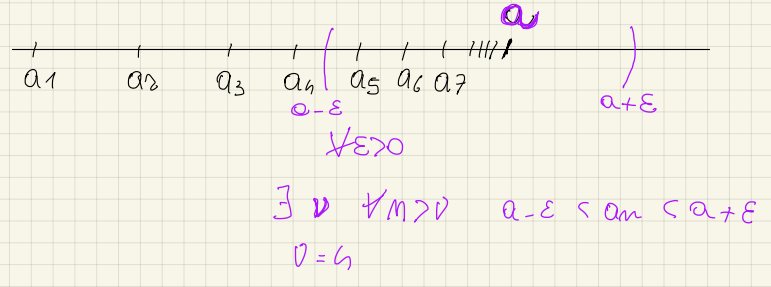
\includegraphics[width=0.3\textwidth]{4.png}
    \caption{Intorno}
    \label{fig:4}
\end{figure}
$a$ è il limite della successione se comunque si scelga un intervallo di numeri intorno ad $a$, diciamo $(a-\varepsilon, a+\varepsilon), \ \varepsilon > 0$, allora esiste un indice $\nu$, tale che $\forall n > \nu \ a_n$ sta nell'intervallo $(a-\varepsilon, a+\varepsilon)$, cioè $a-\varepsilon < a_n < a+\varepsilon$.

\subsection{Limiti}
Un numero reale $a$ è il limite della succesione $a_n$ (si dice che $a_n$ tende
o converge ad $a$) e si scrive:
\[
    \lim_{n\to +\infty} a_n = a \ \ \text{ o } a_n \to_{n\to+\infty} a
\]
se, qualunque sia $\varepsilon > 0$, esiste un numero $\nu$ tale che:
\[
    |a_n - a| < \varepsilon \ \ \ \ \forall n > \nu
\]
In simboli:
\[
    \lim_{n\to+\infty}a_n = a \iff \forall \varepsilon > 0 \ \ \ \ \exists \nu \in \mathbb{N} : |a_n - a| < \varepsilon \ \ \ \ \forall n > \nu
\]
\textbf{Osservazione:} $a-\varepsilon < a_n < a+\varepsilon$ si può scrivere $-\varepsilon < a_n - a < \varepsilon$.\\
% In generale vale la seguente preposizione:
% \subsubsection{Proposizione}
% Per ogni numero reale $\nu\geq 0$
% \[
%     |x| \leq \nu \iff -\nu \leq x \leq \nu
% \]
% \[
%     |x| < \nu \iff -\nu < x < \nu
% \]
\subsection{Proposizione}
Se esiste il limite $a\in\R$ della successione $a_n$, allora è unico.\\
\textbf{Dimostrazione:} Ragioniamo per assurdo. Supponiamo che:
\[
    a_n \to a \ \ \ \ \text{ e } \ \ \ \ a_n \to b \ \ \ \ \text{ con } a \neq b
\]
Allora $\forall\varepsilon > 0$
\[
    \exists \nu_1 : |a_n - a| < \varepsilon \ \ \ \ \forall n > \nu_1
\]
\[
    \exists \nu_2 : |a_n - b| < \varepsilon \ \ \ \ \forall n > \nu_2
\]
Prendo $\varepsilon = \dfrac{|a-b|}{2} > 0$ e ponendo $\nu = \max\{\nu_1,
    \nu_2\}$, $(1) \text{ e } (2)$ valgono contemporaneamente. Allora:
\[
    |a-b| = |(a-a_n) + (a_n-b)| \leq |a-a_n| + |a_n-b| < \varepsilon + \varepsilon = |a-b|
\]
Ma allora $|a-b| < |a-b|$, ASSURDO! $\clubsuit$ \\ Una succesisone $a_n$ ha
limite $+\infty$ (si dice anche che tende o diverge a $+\infty$)
\[
    \lim_{n\to+\infty}a_n = +\infty \]
se, qualunque sia $M > 0 \in \R$, esiste un numero $\nu$ tale che:
\[
    a_n > M \ \ \ \ \forall n > \nu
\]
In simboli:
\[
    \lim_{n\to+\infty}a_n = +\infty \iff \forall M > 0 \ \ \ \ \exists \nu \in \mathbb{N} : a_n > M \ \ \ \ \forall n > \nu
\]
Analogamente si definisce il limite $-\infty$:
\[
    \lim_{n\to+\infty}a_n = -\infty \iff \forall M < 0 \ \ \ \ \exists \nu \in \mathbb{N} : a_n < M \ \ \ \ \forall n > \nu
\]
\textbf{Osservazione:} \begin{itemize}
    \item Le successioni che ammettono limite finito si dicono \textbf{convergenti}
    \item Le successioni che ammettono limite infinito si dicono \textbf{divergenti}
    \item Le successioni convergenti o divergenti si dicono \textbf{regolari}
    \item Una successione che tende a zero si dice anche \textbf{infinitesima}
    \item Una successione divergente si dice anche \textbf{infinita}
\end{itemize}

\subsection{Successioni Limitate}
$a_n$ si dice \textbf{limitata} se $\exists M\in\R \ : $
\[
    |a_n| \leq M
\]
\textbf{Osservazione:} In particolare $a_n = (-1)^n$ è un esempio di successione limitata che non ammette limite. Viceversa, ogni successione che ammette limite finito, è limitata. Vale il seguente:
\subsection{Teorema}
Ogni successione convergente è limitata.\\ \textbf{Dimostrazione:} Sia $a_n$
una successione convergente e supponiamo che:
\[
    \lim_{n\to+\infty}a_n = a
\]
Allora $\forall\varepsilon > 0 \ \ \ \ \exists \nu \in \mathbb{N} : |a_n - a| <
    \varepsilon \ \ \ \ \forall n > \nu$\\ Posso predere $\varepsilon = 1 \implies
    |a_n - a|<1$, valuto $|a_n|$:
\[
    |a_n| = |(a_n-a) + a| \leq |a_n-a| + |a| < 1 + |a| \ \ \ \ \forall n > \nu
\]
posso prendere $M = \max\{|a_1|, |a_2|, \cdots, |a_\nu|, 1+|a|\} \ \
    \clubsuit$.

\subsection{Operazioni con i limiti}
Supponiamo $\lim_{n\to+\infty} a_n = a$ e $\lim_{n\to+\infty} b_n = b$ con $a,
    b \in \R$. Allora:
\begin{itemize}
    \item $\lim_{n\to+\infty} (a_n + b_n) = a + b$
    \item $\lim_{n\to+\infty} (a_n - b_n) = a - b$
    \item $\lim_{n\to+\infty} (a_n \cdot b_n) = a \cdot b$
    \item $\lim_{n\to+\infty} \dfrac{a_n}{b_n} = \dfrac{a}{b}$ se $b \neq 0$
\end{itemize}
Si dimostra anche che:
\begin{itemize}
    \item $a_n \to a \ b_n \to \pm\infty \implies a_n + b_n \to \pm\infty$
    \item $a_n \to a (\ne0) \ b_n \to\pm\infty \implies a_n\cdot b_n \to \pm\infty$
    \item $a_n \to a \ b_n \to \pm\infty$ entrambe con lo stesso segno $\implies a_n + a_b \to \pm\infty$ e $a_n\cdot b_n \to +\infty$
    \item $a_n \to a \ b_n\to\pm\infty \implies \dfrac{a_n}{b_n} \to 0$
    \item $a_n \to \pm a \ b_n \to \pm0 \implies \dfrac{a_n}{b_n} \to +\infty$
\end{itemize}

\subsection{Forme infeterminate o di indecisione}
\begin{itemize}
    \item $\infty - \infty$
    \item $0 \cdot \infty$
    \item $\dfrac{\infty}{\infty}$
    \item $\dfrac{0}{0}$
    \item $\infty^0$
    \item $1^{\pm\infty}$
    \item $0^0$
\end{itemize}
Dire che un limite è una forma indeterminata non significa dire che non esiste, ma che occorre togliere, se possibile, l'indeterminazione, mediante semplificazioni o trasformazioni.
\subsection{Teoremi di confronto}
\subsubsection{Teorema della permanenza del segno}
Se $\lim_{n\to+\infty} a_n = a > 0$, esiste un numero $\nu$ tale che $a_n > 0 \
    \ \ \ \forall n > \nu$.\\ \textbf{Esempio:} $a_n = \dfrac{n-12}{n}$,
$\lim_{n\to+\infty} a_n = 1 > 0$, ma i primi termini della successione sono
negativi.\\ $a_n = 0$ per $n = 12$, quindi se prendo $\nu = 12$, e $n > \nu$
allora $a_n > 0$.\\ \textbf{Dimostrazione:} $\lim_{n\to+\infty} a_n = a \iff
    \forall\varepsilon>0 \ \ \ \ \exists\nu\in\mathbb{N} : |a_n - a| < \varepsilon
    \ \ \ \ \forall n > \nu$\\ $a > 0$, quindi posso prendere $\varepsilon =
    \dfrac{a}{2} > 0$ e:
\[
    |a_n - a| < \dfrac{a}{2} \ \ \ \forall n > \nu \iff -\dfrac{a}{2} < a_n - a < \dfrac{a}{2} \ \ \ \ \forall n > \nu \iff a_n > a - \dfrac{a}{2} = \dfrac{a}{2} > 0 \ \ \ \ \forall n > \nu \ \ \ \clubsuit
\]
\subsubsection*{Corollario (viceversa)}
Se $\lim_{n\to+\infty} a_n = a$ e $a_n \geq 0$ (vale anche $a_n > 0$), allora
$a \geq 0$.

\subsubsection{Teorema dei carabinieri}
Si consideriamo tre successioni $a_n, b_n, c_n$ con la proprietà che:
\[
    a_n \leq c_n \leq b_n
\]
Se risulta che $\lim_{n\to+\infty} a_n = \lim_{n\to+\infty} b_n = a$, allora
anche $\lim_{n\to+\infty} c_n = a$ (per ipotesi $a_n \to a \ \ b_n \to a$).\\
\textbf{Dimostrazione:}
\[
    \forall\varepsilon>0 \ \ \exists\nu_1 : |a_n - a| < \varepsilon \ \ \forall n > \nu_1
\]
\[
    \forall\varepsilon>0 \ \ \exists\nu_2 : |b_n - a| < \varepsilon \ \ \forall n > \nu_2
\]
Definisco $\nu_3 = \max\{\nu_1, \nu_2\}$ e per ipotesi $a-\varepsilon < a_n
    \leq c_n \leq b_n < a+\varepsilon \implies |c_n - a| < \varepsilon \ \ \forall
    n > \nu_3 \ \ \implies c_n \to a \ \ \clubsuit$ \textbf{Osservazione:} Valgono
per i limiti infiniti:
\[
    a_n \leq b_n \ \ \ \forall n\in \mathbb{N} \begin{cases}
        a_n\to+\infty \implies b_n\to+\infty \\
        b_n\to-\infty \implies a_n\to-\infty
    \end{cases}
\]
Dal teorema dei Carabinieri, segue il seguente risultato molto importante per
le applicazioni e gli esercizi:
\subsubsection{Teorema del limite del prodotto di una successione limitata per una infinitesima}
Se $a_n$ è limitata e $b_n$ è infinitesima, allora $a_n\cdot b_n \to 0$
\textbf{Dimostrazione:} Considero $|a_n\cdot b_n| \implies$
\[
    |a_n\cdot b_n| = |a_n|\cdot|b_n| \leq M\cdot|b_n|
\]
Per la proprietà del valore assoluto $|x| \leq r \iff -r \leq x \leq r$\\
\[
    -M|b_n| \leq a_n\cdot b_n \leq M|b_n| \ \ \ \text{ per ipotesi } b_n\to0
\]
$\implies$ Per il Teorema dei Carabinieri $a_n\cdot b_n \to 0 \ \ \ \clubsuit$

\subsection{Alcuni limiti notevoli}
\begin{itemize}
    \item $\lim_{n\to\infty}a^n = \begin{cases}
                  +\infty \ \ \ \ \text{ se } a > 1 \\
                  0 \ \ \ \ \text{ se } -1 < a < 1
                  1 \ \ \ \ \text{ se } a = 1
                  \text{non esiste} \ \ \ \ \text{ se } a \leq -1
              \end{cases}$
    \item $\lim_{n\to\infty}n^b = \begin{cases}
                  +\infty \ \ \ \ \text{ se } b > 0 \\
                  1 \ \ \ \ \text{ se } b = 0
                  0 \ \ \ \ \text{ se } b < 0
              \end{cases}$
    \item $\lim_{n\to+\infty}\sqrt[n]{a} = \lim_{n\to+\infty}a^{\frac{1}{n}} = 1 \ \ \ \ \forall a > 0$
    \item $\lim_{n\to+\infty}\sqrt[n]{n^b} = \lim_{n\to+\infty}n^{\frac{b}{n}} = 1 \ \ \ \ \forall b \in \R$
\end{itemize}

\subsection{Limiti relativi alle funzioni trigonometriche}
\begin{itemize}
    \item $a_n\to0 \implies \sin a_n \to 0$
    \item $a_n\to0 \implies \cos a_n \to 1$
\end{itemize}
Ad esempio, se $a_n = \frac{1}{n} \implies \sin\frac{1}{n} \to 0$ e $\cos\frac{1}{n} \to 1$.
\begin{itemize}
    \item $a_n\to0, a_n\ne0 \ \ \forall n \ \ (1) \dfrac{\sin a_n}{a_n} \to 1$
    \item $a_n\to0, a_n\ne0 \ \ \forall n \ \ (2) \dfrac{1-\cos a_n}{a_n^2} \to \dfrac{1}{2}$
\end{itemize}
Infatti $\dfrac{1-\cos a_n}{a_n^2} = \dfrac{(1-\cos a_n)(1+\cos a_n)}{a_n^2(1+\cos a_n)} = \dfrac{1-\cos^2 a_n}{a_n^2(1+\cos a_n)} = \dfrac{\sin^2 a_n}{a_n^2}\cdot \dfrac{1}{1+\cos a_n} = \dfrac{1}{2}$

\subsection{Successione notevole importante}
\[
    a_n = (1+\dfrac{1}{n})^n \ \ \ \ 1^{+\infty}
\]
Confrontiamola con altre successioni $b_n, c_n$:
\[
    b_n = (1+\dfrac{1}{n})^3 = (1+\dfrac{1}{n})\cdot(1+\dfrac{1}{n})\cdot(1+\dfrac{1}{n})\to 1
\]
\[
    c_n = (1+\dfrac{1}{10})^n = (\dfrac{11}{10})^n = a^n \to +\infty \ \ \ \ \text{ con } a > 1
\]
Quindi $a_n$ è una \textbf{forma indeterminata} $1^{+\infty}$, che da una
parte, vuole tendere ad 1, dall'altra a $+\infty$, arriverà quindi ad un `punto
di mezzo'. Si definisce $e$ il \textbf{numero di Nepero} tale che:
\[
    e = \lim_{n\to+\infty}(1+\dfrac{1}{n})^n
\]
dove $e \simeq 2,718281828459\ldots$\\ Si dimsotra che la succesisone $a_n$ è
strettamente crescente e limitata.

\subsection{Successioni Monotòne}
\begin{itemize}
    \item $a_n$ strettamente crescente $\iff a_n < a_{n+1} \ \ \ \ \forall n \in \mathbb{N}$
    \item $a_n$ strettamente decrescente $\iff a_n > a_{n+1} \ \ \ \ \forall n \in \mathbb{N}$
    \item $a_n$ crescente $\iff a_n \leq a_{n+1} \ \ \ \ \forall n \in \mathbb{N}$
    \item $a_n$ decrescente $\iff a_n \geq a_{n+1} \ \ \ \ \forall n \in \mathbb{N}$
\end{itemize}
Una successione si dice \textbf{monotona} se si verifica una delle quattro condizioni.\\
Una successione si dice \textbf{costante} se $a_n = a \ \ \ \ \forall n \in \mathbb{N}$ con $a$ numero reale. Le successioni costanti sono sia crescenti che decrescenti.

\subsection{Teorema sulle successioni monotone}
Ogni successione monotona ammette limite. In particolare, ogni successio
monotona e limitata ammette limite finito.\\ \textbf{Osservazione:}
Naturalmente non è che ogni successione convergente è monotona. Ad esempio $an
    = \frac{(-1)^n}{n}$ è convergente ($\to 0$), ma non è monotona.\\
\textbf{Dimostrazione:} $(1)$ Sia, ad esempio, $a_n$ crescente e limtata.\\
Poniamo $l = \sup a_n$ (teorema di esistenza dell'estremo superiore: esiste il
sup ed è finito perchè $a_n$ è limitata).\\ Allora, per le proprietà
dell'estremo superiore (data che è il minimo dei maggioranti)
\[
    \forall\varepsilon>0 \ \ \ \ \exists \nu : l-\varepsilon < a_\nu \ \ (\star)
\]
Ma $a_n$ è monotona (crescente), quindi $\forall n>\nu \ \ \ a_\nu \leq a_n$,
da $(\star)$
\[
    l-\varepsilon < a_\nu \leq a_n \leq l < l+\varepsilon \ \ \ \ \forall n > \nu
\]
\[
    |a_n - l| < \varepsilon \ \ \ \ \forall n > \nu
\]
$\implies \lim_{n\to+\infty}a_n = l \ \ \ \clubsuit$\\
$(2)$ Sia ora $a_n$ crescente e non limitata. Fissiamo $M > 0$, allora esiste $\nu$ tale che $a_\nu > M$. Dato che $a_n$ è crescente $\forall n>\nu$
\[
    a_n \geq a_\nu > M
\]
$\implies \lim_{n\to+\infty}a_n = +\infty \ \ \ \clubsuit$\\
\textbf{Osservazione:} Assioma di completezza $\implies$ Esistenza dell'estremo superiore $\implies$ Esistenza del limite delle successioni monotone\\
\textbf{Osservazione:} Si dimostra che $a_n = (1+\frac{1}{n})^n$ è strettamente crescente e limitata. Quindi esiste, ed è un numero reale, il limite per $n\to+\infty$ di $a_n$, che è $e$.

\subsection{Limiti Notevoli}
\begin{itemize}
    \item $\lim_{n\to+\infty} (1+\dfrac{1}{n})^n = e$
    \item $\lim_{n\to+\infty} (1+\dfrac{x}{n})^n = e^x$ con $x \in \R$
\end{itemize}
Più in generale:
\begin{itemize}
    \item $\lim_{n\to+\infty} (1+\dfrac{x}{a_n})^a_n = e^x$ con $a_n \to +\infty$, $x \in \R$
    \item $\lim_{n\to+\infty} (1+\varepsilon n)^{\frac{1}{\varepsilon}} = e$ con $\varepsilon \to 0$
    \item $\lim_{n\to+\infty} (1+x\varepsilon n)^{\frac{1}{\varepsilon}} = e^x$ con $\varepsilon \to 0$, $x \in \R$
\end{itemize}
\textbf{Osservazione:} Abbiamo visto, nell'ambito dei \textbf{limiti notevoli}, la successione esponenziale $a^n$, con $a > 1$ e la successione potenza $n^b$, con $b > 0$.\\
Entrambe divergono a $+\infty$. Spesso tali successioni vengono confrontate con $\log n, n!$ e con $n^n$, che pure divergono a $+\infty$.\\

\subsubsection{Infiniti di ordine crescente}
$\log n$, $n^b$, $a^n$, $n!$, $n^n$, da cui:
\begin{itemize}
    \item $\lim_{n\to+\infty} \dfrac{\log n}{n^b} = 0$
    \item $\lim_{n\to+\infty} \dfrac{a^n}{n!} = 0$
    \item $\lim_{n\to+\infty} \dfrac{n!}{n^n} = 0$
    \item $\lim_{n\to+\infty} \dfrac{n^b}{a^n} = 0$
\end{itemize}

\subsection{Criterio del rapporto per le successioni}
Sia $a_n$ una successione a termini positivi.\\ Sia $\dfrac{a_n+1}{a_n} \to a$,
se $a \in [0, 1)$, allora la successione $a_n$ converge a zero.\\ Se $a \in (1,
    +\infty)$, allora la successione $a_n$ diverge a $+\infty$.\\
\textbf{Osservazione:} Il caso $a = 1$ non è contemplato nell'enunciato.

\subsection{Successioni estratte}
Considero $a_n$ successione di numeri reali e sia $n_k$ una successione
strettamente crescente di numeri naturali.\\ La successione $a_{nk}$
\[
    k\in\mathbb{N} \to a_{n_k}
\]
prende il nome di \textbf{successione estratta da $a_n$} di inidici $n_k$.\\
\textbf{Osservazione:} Si dimostra che se $a_n$ converge ad $a$, allora ogni
successione estratta $a_{n_k}$ converge ad $a$.\\ \textbf{Osservazione:}
Abbiamo dimostrato che ogni successione $a_n$ convergente è limitata. Il
viceversa non è vero, ma vale il seguente notevole risultato:

\subsection{Teorema di Bolzano-Weierstrass}
Sia $a_n$ una successione limitata. Allora esiste almeno una sua estratta
convergente.

\end{document}